\section{Experiments}
\label{sec:experiments}







\subsection{Main Results}
\label{sec:main-results}
 
\paragraph{PowerOPD substantially outperforms vanilla OPD.}
PowerOPD consistently improves over vanilla OPD across all four teacher--student configurations (Tables~\ref{tab:main} and~\ref{tab:main-1p7b}). Averaged over configurations using the best PowerOPD variant for each metric, PowerOPD improves the mean performance by \(\mathbf{+4.47}\) Avg@8 and \(\mathbf{+4.06}\) Pass@8. The largest benchmark-averaged gain occurs in the Qwen3-4B \(\to\) Qwen3-0.6B-Base setting, with Avg@8 improving from 19.13 to 25.50 (\(\mathbf{+6.37}\)) and Pass@8 from 36.18 to 41.89 (\(\mathbf{+5.71}\)). Gains also hold for the Qwen3-8B \(\to\) Qwen3-0.6B-Base setting (\(+3.87\) Avg@8, \(+3.62\) Pass@8), the Qwen3-4B \(\to\) Qwen3-1.7B-Base setting (\(+5.04\) Avg@8, \(+4.39\) Pass@8), and the Qwen3-8B \(\to\) Qwen3-1.7B-Base setting (\(+2.60\) Avg@8, \(+2.53\) Pass@8). On individual benchmarks, the gains are larger, reaching up to \(\mathbf{+16.75}\) Avg@8 on AMC23 in the Qwen3-4B \(\to\) Qwen3-0.6B-Base setting and \(\mathbf{+15.00}\) Pass@8 on AMC23 in the Qwen3-4B \(\to\) Qwen3-1.7B-Base and Qwen3-8B \(\to\) Qwen3-1.7B-Base settings. Notably, \emph{PowerOPD plugs directly into the standard OPD pipeline without modifying rollout generation, teacher scoring, or policy-gradient optimization}.

\begin{table}[t]
  \centering
  \footnotesize
  \setlength{\tabcolsep}{3pt}
  \begin{adjustbox}{max width=\columnwidth}
    \begin{tabular}{lccc}
    \toprule
    \textbf{Method} & \textbf{TFLOPs/upd.} & \textbf{Time/step} & \textbf{Peak mem.} \\
    \midrule
    Full-vocab OPD & 402.7 & 22.14s & 78.99 GiB \\
    PowerOPD & 346.6 & 9.03s & 60.72 GiB \\
    \midrule
    Reduction & $\downarrow$13.9\% & $\downarrow$59.2\% & $\downarrow$23.1\% \\
    \bottomrule
  \end{tabular}
  \end{adjustbox}
  \vspace{-5pt}
  \caption{Efficiency comparison on Qwen3-0.6B-Base $\leftarrow$ Qwen3-4B. Wall-time is averaged over 1.5k training steps; peak memory is measured with batch size 8.}
  \vspace{-12pt}
  \label{tab:efficiency}
\end{table}

\paragraph{PowerOPD also surpasses post-hoc stabilization methods.}
PowerOPD also outperforms post-hoc log-reward stabilization baselines (Tables~\ref{tab:main} and~\ref{tab:main-1p7b}). The largest benchmark-averaged gain occurs in the Qwen3-4B \(\to\) Qwen3-0.6B-Base setting, where PowerOPD improves over the strongest post-hoc baseline from 22.49 to 25.50 Avg@8 (\(\mathbf{+3.01}\)) and from 38.35 to 41.89 Pass@8 (\(\mathbf{+3.54}\)). At the individual-benchmark level, the gains reach up to \(\mathbf{+8.43}\) Avg@8 and \(\mathbf{+7.50}\) Pass@8 on AMC23 in the same setting. Notably, \emph{Z-Score} can underperform vanilla OPD, consistent with our analysis in \secref{sec:properties} that batch centering may violate sign consistency. These results show that post-hoc stabilization is insufficient: \emph{the reward properties must hold at the probability-to-reward mapping level, before the log-ratio distortion occurs.}

\begin{figure*}[t]
  \centering
  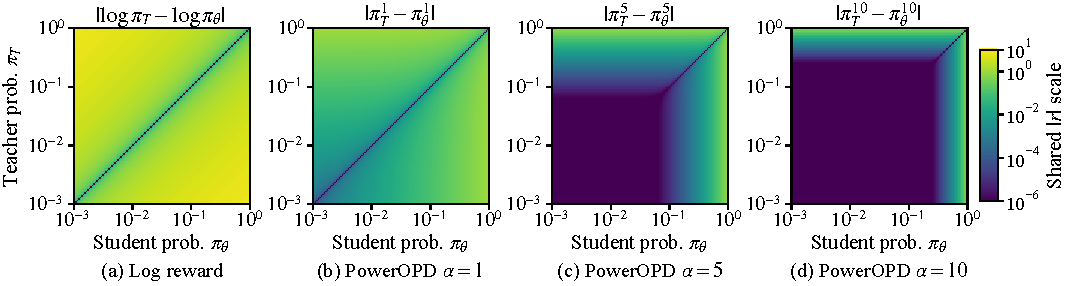
\includegraphics[width=\textwidth]{figures/alpha_heatmap.pdf}
  % \vspace{-20pt}
    \caption{Reward magnitude over the joint probability space $(\pi_T, \pi_\theta)$. (a) The log-ratio reward depends only on the ratio $\pi_T/\pi_\theta$: it retains full sensitivity where both probabilities are small and grows without bound as either approaches zero. (b--d) PowerOPD couples reward magnitude to the absolute probability level: as $\alpha$ grows, the inert region expands and the signal contracts toward tokens with substantial probability under at least one model.}
  \label{fig:alpha-heatmap}
  \vspace{-10pt}
\end{figure*}

\begin{figure}[t]
  \centering
  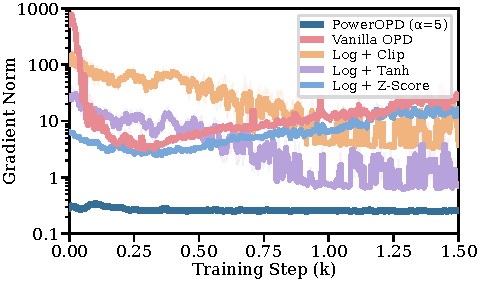
\includegraphics[width=\columnwidth]{figures/fig5_gradnorm_stability.pdf}
  % \vspace{-20pt}
    \caption{
    Gradient norm during training with a Qwen3-1.7B-Base student and Qwen3-4B teacher.
    }
    \label{fig:stability}
  % \vspace{-3pt}
  
\end{figure}

% \begin{figure}[t]
%   \centering
%   \begin{minipage}[t]{0.49\columnwidth}
%     \centering
%     \includegraphics[width=\linewidth]{figures/fig6a_reward_bucket_abs.pdf}\\[-0.5ex]
%     \textbf{(a)}
%   \end{minipage}\hfill
%   \begin{minipage}[t]{0.49\columnwidth}
%     \centering
%     \includegraphics[width=\linewidth]{figures/fig6b_reward_bucket_signed.pdf}\\[-0.5ex]
%     \textbf{(b)}
%   \end{minipage}
%   \vspace{-6pt}
%     \caption{
%     Reward statistics by student-probability bucket: (a) mean absolute reward and (b) signed mean reward for OPD and PowerOPD across \(\alpha\).
%     }   
%     \label{fig:sensitivity}
%     \vspace{-10pt}
    
% \end{figure}

\paragraph{PowerOPD consistently outperforms full-vocabulary OPD at substantially lower compute cost.}
Taking the best PowerOPD variant separately for each metric, the largest benchmark-averaged gains are \(\mathbf{+2.59}\) Avg@8 and \(\mathbf{+8.90}\) Pass@8. Specifically, with the Qwen3-0.6B-Base student, PowerOPD improves Avg@8 by \(+2.59\) and \(+0.56\) over full-vocabulary OPD under the 4B and 8B teachers, with corresponding Pass@8 gains of \(+8.17\) and \(+8.90\). With the Qwen3-1.7B-Base student, PowerOPD improves Avg@8 by \(+1.86\) and \(+1.22\), and Pass@8 by \(+2.29\) and \(+2.98\), under the 4B and 8B teachers, respectively. At the individual-benchmark level, the gains are substantially larger, reaching up to \(\mathbf{+11.60}\) Avg@8 on Olympiad in the Qwen3-4B \(\to\) Qwen3-0.6B-Base setting and \(\mathbf{+25.00}\) Pass@8 on AMC23 in the Qwen3-8B \(\to\) Qwen3-0.6B-Base setting. As shown in \autoref{tab:efficiency}, PowerOPD reduces wall-clock time by \(59.2\%\) and peak GPU memory by \(23.1\%\), with FLOPs computation detailed in \autoref{app:flops}. These results show that a bounded sampled-token reward can surpass full-vocabulary distillation while avoiding vocabulary-wide computation.
 
\paragraph{PowerOPD scales with larger \(\alpha\).}
Across all configurations, increasing \(\alpha\) generally improves Avg@8 and Pass@8 while shortening responses. In the 0.6B/4B setting, Avg@8 rises from 24.16 at \(\alpha{=}0.1\) to 25.50 at \(\alpha{=}500\), Pass@8 from 39.61 to 41.89, and average length drops from 2{,}291 to 1{,}875 tokens. The same trend holds in the 1.7B/4B setting, where Avg@8 improves from 33.89 to 36.02 and length decreases from 1{,}900 to 1{,}579 tokens. This suggests that larger \(\alpha\) encourages more targeted responses rather than longer generations. In contrast, full-vocabulary OPD often saturates the 4,096-token limit, consistent with the length inflation observed by \citet{luo2026demystifying}, 
indicating weaker length calibration despite strong accuracy. Notably, PowerOPD scales with \(\alpha\) without any additional supervision.



\subsection{Analysis}
\paragraph{Training Dynamics Across \texorpdfstring{\(\alpha\)}{alpha}}
\label{subsec:alpha-training-dynamics}

We conduct a fine-grained sweep over \(\alpha\) to study how the PowerOPD reward shape affects training dynamics. As shown in \autoref{fig:alpha}, we compare PowerOPD with vanilla OPD and full-vocabulary OPD under the Qwen3-0.6B-Base student with Qwen3-4B and Qwen3-8B teachers. First, \emph{larger \(\alpha\) leads to faster and stronger convergence.} Vanilla OPD exhibits the delayed-improvement phase diagnosed earlier and converges to a weaker final accuracy, whereas PowerOPD reaches high validation accuracy much earlier in training; larger \(\alpha\) further improves both convergence speed and final accuracy. Second, \emph{larger \(\alpha\) yields shorter and more stable generations.} As \(\alpha\) increases, PowerOPD drives the student toward shorter responses and stabilizes earlier, while vanilla OPD remains length-unstable and can fail to settle into a stable generation regime. Full-vocabulary OPD also often approaches the maximum generation length, indicating that stronger accuracy does not necessarily translate into better length calibration.

\paragraph{Why Larger \texorpdfstring{\(\alpha\)}{alpha} Improves PowerOPD}
\label{subsec:reward-sensitivity}

% \secref{sec:poweropd} suggests that larger \(\alpha\) suppresses low-probability reward sensitivity and shifts learning toward better-supported tokens. We verify this in the Qwen3-0.6B-Base student and Qwen3-4B teacher setting by grouping sampled rollout tokens into four student-probability buckets: \([0,0.01)\), \([0.01,0.1)\), \([0.1,0.5)\), and \([0.5,1.0]\). \autoref{fig:sensitivity}(a) shows that the log-ratio reward assigns extreme magnitudes to low-probability tokens, while larger \(\alpha\) suppresses them; \autoref{fig:sensitivity}(b) shows that these signals are dominated by strong negative rewards, which also become milder as \(\alpha\) increases. This selective suppression helps in two ways: (i)~\emph{it reduces rare-event variance}, since low-probability samples are rare Monte Carlo events and large rewards create high-leverage policy-gradient terms \(r_t\nabla_\theta\log\pi_\theta(o_t\mid c_t)\)~\citep{williams1992reinforce,greensmith2004variance,schulman2018highdimensionalcontinuouscontrolusing}; and (ii)~\emph{it avoids over-correcting marginal behaviors}, since low-probability tokens are not dominant modes of the policy but can dominate the update under extreme rewards. Thus, larger \(\alpha\) preserves the teacher-aligned optimization direction while preventing rare low-probability tokens from dominating updates, explaining faster accuracy convergence and more stable length dynamics in \autoref{fig:alpha}.
To understand why larger $\alpha$ improves accuracy, we examine how the reward distributes its magnitude over the joint probability space $(\pi_T, \pi_\theta)$ in \autoref{fig:alpha-heatmap}. The log-ratio reward depends only on the ratio $\pi_T/\pi_\theta$ and is blind to the absolute probability level: it assigns the same reward to $0.002$ versus $0.0001$ as to $0.2$ versus $0.01$, and grows without bound whenever one probability approaches zero while the other does not (\autoref{fig:alpha-heatmap}(a)). Consequently, its most extreme values fall on tokens that are improbable under both models, where the student rarely samples the token and the probability estimates carry the least statistical support, creating high-leverage policy-gradient terms $r_t \nabla_\theta \log \pi_\theta(o_t \mid c_t)$ from the least reliable measurements~\citep{williams1992reinforce, greensmith2004variance}. PowerOPD couples the reward magnitude to the absolute probability level: $|r_t^{\alpha}|$ is governed by $\max(\pi_T, \pi_\theta)^{\alpha}$, so a token receives substantial reward only if at least one model assigns it substantial probability, and $\alpha$ sets how strict this support requirement is. At $\alpha{=}1$, a probability of $0.6$ retains a sizable reward, whereas at $\alpha{=}10$ it contributes only $0.6^{10} \approx 0.006$. Accordingly, in \autoref{fig:alpha-heatmap}(b--d), the inert region expands as $\alpha$ grows, and the surviving signal contracts toward tokens where the teacher probability is high, so the distillation target is reliable, or the student probability is high, so the update adjusts the dominant modes of the current policy rather than its marginal behaviors. Larger $\alpha$ therefore suppresses exactly the unreliable high-leverage tokens that destabilize vanilla OPD (\secref{subsec:high-variance}), while concentrating learning on well-supported ones.

\paragraph{Training Stability}
\label{subsec:training-stability}

We further assess training stability by tracking gradient norms with a Qwen3-1.7B-Base student and Qwen3-4B teacher. As shown in \autoref{fig:stability}, vanilla OPD has an initial spike near \(10^3\) and later rises above \(20\), reflecting instability from high-variance log-ratio rewards. Post-hoc methods only partially mitigate this behavior: \emph{Clip} and \emph{Tanh} still fluctuate sharply, often exceeding \(10\), while \emph{Z-Score} grows from around \(3\) to above \(10\). In contrast, PowerOPD keeps the gradient norm nearly flat at \(0.25\)--\(0.35\), about \(3{,}000\times\) smaller than the initial OPD spike, over \(60\times\) smaller than late-stage OPD, and over \(30\times\) smaller than the high-gradient regimes of \emph{Clip} and \emph{Z-Score}. This shows that bounding the reward at the probability-to-reward mapping level stabilizes policy-gradient updates more effectively than post-hoc transformations of the log-ratio reward.